\section{Structures de données}

    \subsection{XML}
        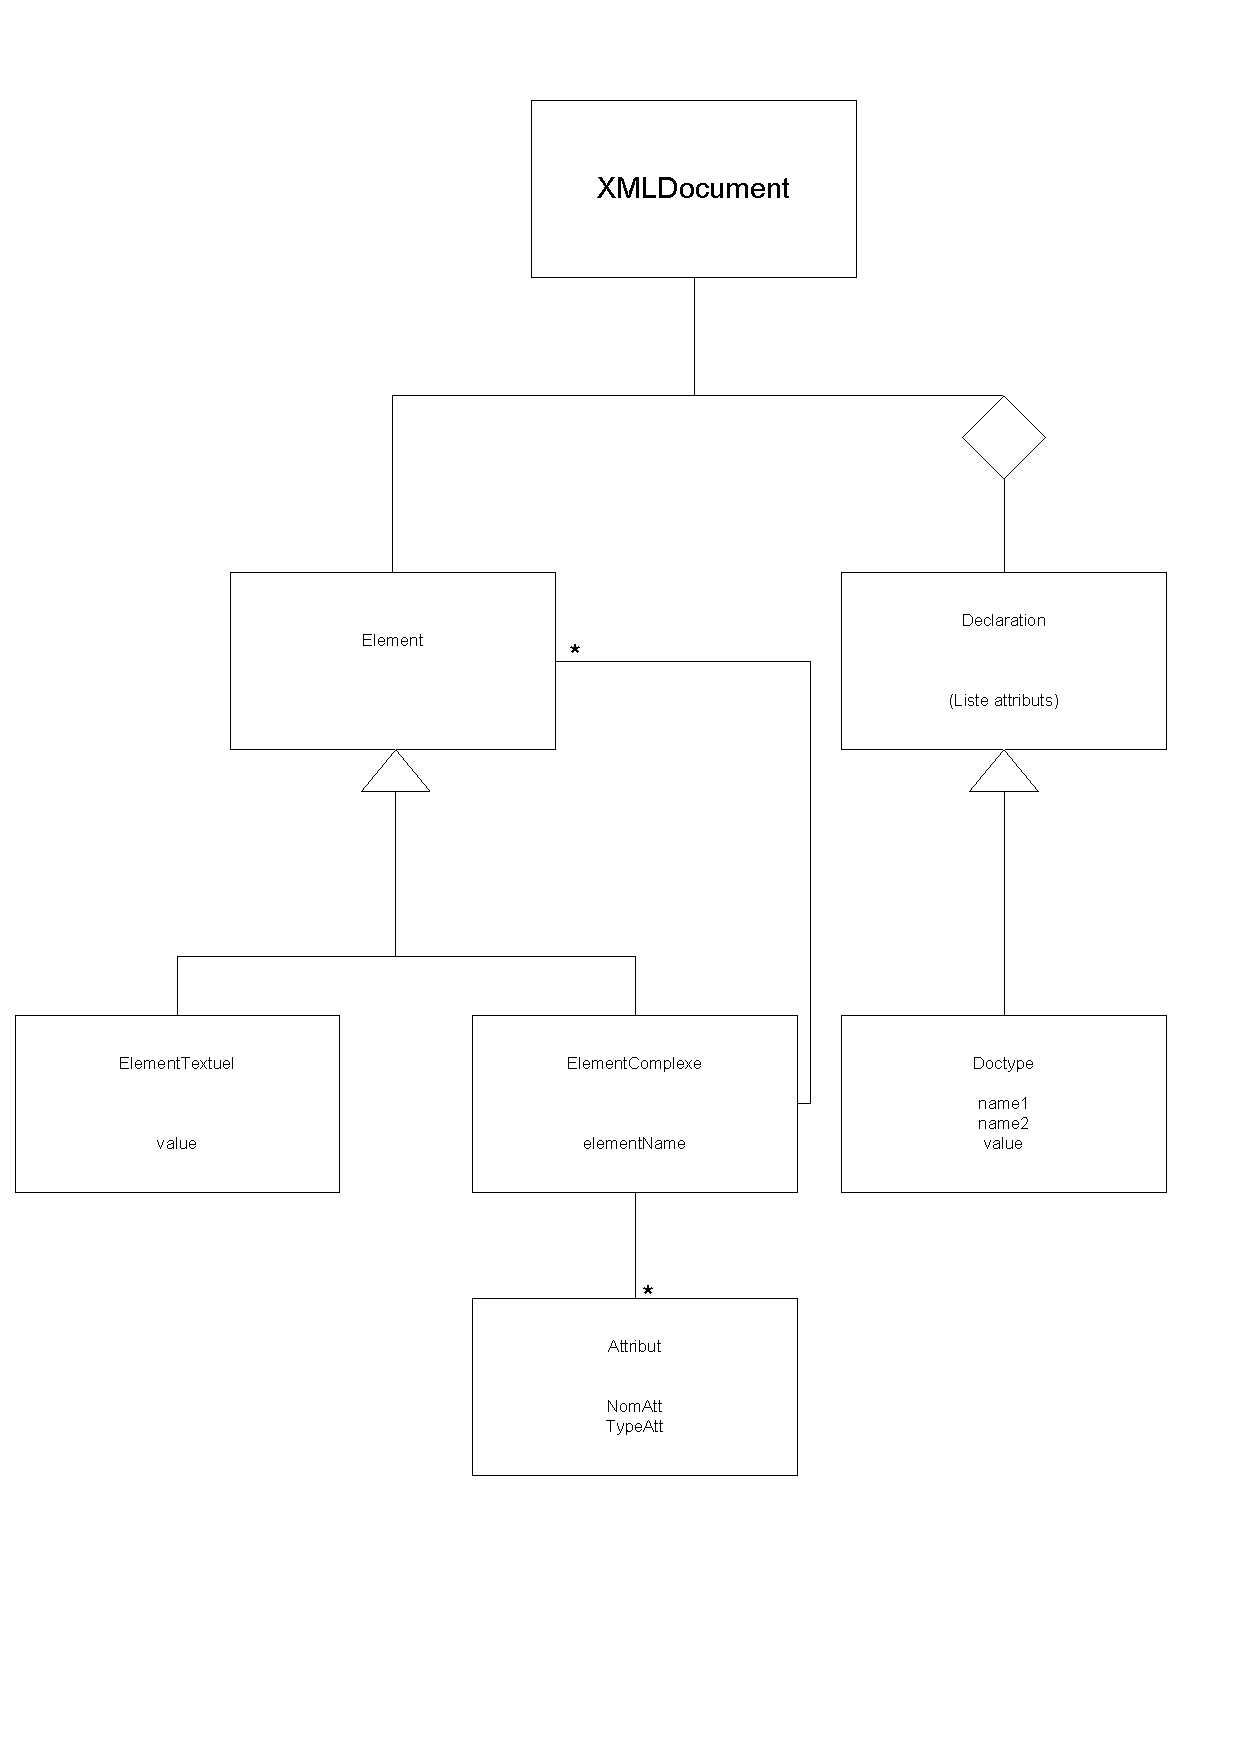
\includegraphics[width=\textwidth]{img/ClassesXML.pdf}\\
        La structure de donnée généré pendant la lecture du XML
        
    \subsection{DTD}
        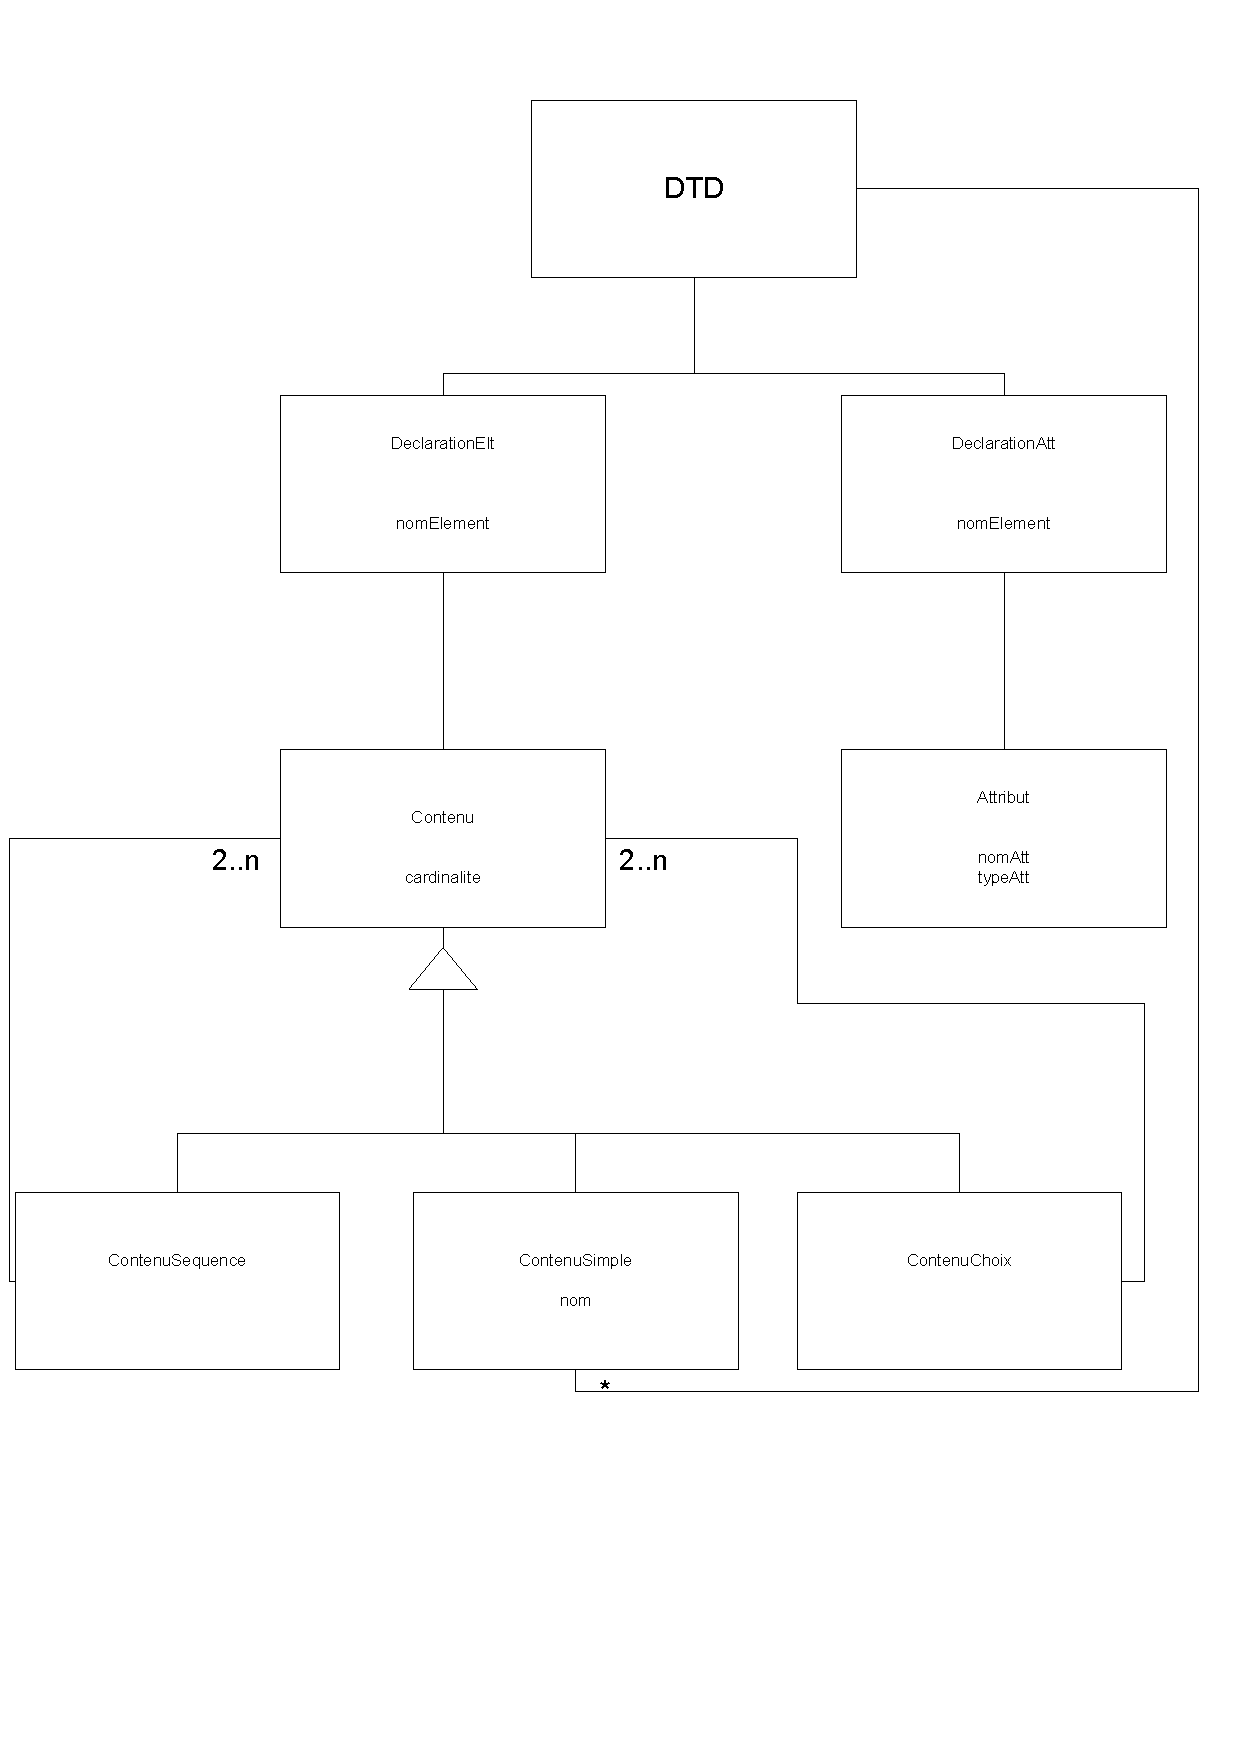
\includegraphics[width=\textwidth]{img/ClassesDTD.pdf}\\
        La structure de donnée généré pendant la lecture de la DTD
        
\section{Algorithmes}

    \subsection{Validation}
	
	ALgorithme de validation :
	
	\begin{algorithm}
	\caption{validateXML(XML $xml$, DTD $dtd$)}
	\begin{algorithmic}
	    \STATE String $exp \gets$ transformXML(xml) \COMMENT{transformer le fichier XML en une expression a valider}
	    \STATE String $pattern \gets$ transformDTD(dtd) \COMMENT{transformer le fichier DTD en pattern}
	    \STATE bool $resultat \gets$ match(exp, pattern) \COMMENT{valider}
    \end{algorithmic}
    \end{algorithm}
    
    \begin{algorithm}
	\caption{transformDTD(DTD dtd)}
    \begin{algorithmic}
	    \RETURN tranformDeclarationElement(dtd.racine) \COMMENT{on commencer par l'element racine}
    \end{algorithmic}
    \end{algorithm}
        
    \begin{algorithm}
	\caption{tranformDeclarationElement(DeclarationElement decEle)}    
    \begin{algorithmic}
	    \STATE String $result$ \COMMENT{transformer recursivement} 
        \IF{$decEle$ est textuel}
		    \STATE $result \gets$ "\textless"+decEle.nom+decATTLIST"\textgreater decText"\textless/"+decEle.nom+"\textgreater
	    \ELSE
		    \STATE $result \gets$ "(\textless"+decEle.nom+decATTLIST"\textgreater"
		    \FOR{chaque element fils $filsEle$}
			    \IF{pas de contraintes de cardinalité}
				    \STATE $result$ += tranformDeclarationElement(filsEle)
			    \ELSE
				    \STATE $result$ += "(" tranformDeclarationElement(filsEle)+cardinalite(filsEle)+")"
		        \ENDIF
	        \ENDFOR
	    \ENDIF
	\end{algorithmic}
    \end{algorithm}
        
    \subsection{Transformation}
    
     Algorithme de transformation XSLT :
    \begin{algorithm}
	\caption{transformation(ArbreXML, arbre XSLT)}    
    \begin{algorithmic}
		\STATE prendre l'element dont l'attribut est "\" du XSLT, pour construire la racine de l'arbre de retour.
		\STATE tranformer(root, XSLT("/"))
	\end{algorithmic}
    \end{algorithm}
	
	\begin{algorithm}
	\caption{transformer(Element, ArbreXSLT)}    
    \begin{algorithmic}
		\STATE Ajouter à l'arbre le XSL de l'élement.
		\STATE Chercher l'element <xsl:apply-templates/>, pour le remplacer par soit:
			\STATE - pour chaque fils, réécrire le contenu XSL de l'élement, et appeler transformation(fils, ) 
			\STATE - le contenu XML de l'élément.
	\end{algorithmic}
    \end{algorithm}
 
	\paragraph{Explication}
	    Il s'agit de parcourir les arbres XML et XSLT de haut en bas de façon indépendante.
	    On commence par pointer sur la racine de l'arbre XML (/). On recherche dans l'arbre XSLT l'élément "template" dont l'attribut "match" est égal à "/".
	    On recopie l'ensemble de ces fils dans l'arbre HTML. Lorsque l'on tombe sur la feuille "apply\_templates", on retourne sur l'arbre XML et on vérifie que l'élément actuellement pointé à des fils. Si c'est le cas on pointe sur le premier fils, et on recommence la même opération. Si l'élément pointé n'a pas de fils alors on inscrit dans l'arbre HTML le contenu de l'élément XML. On remonte ensuite dans l'arbre XML et on passe à l'élément suivant jusqu'à la fin du parcours de l'arbre XML.

	\paragraph{Exemple}
        \begin{center}
	        On pointe sur "rapport" dans l'arbre XML
	        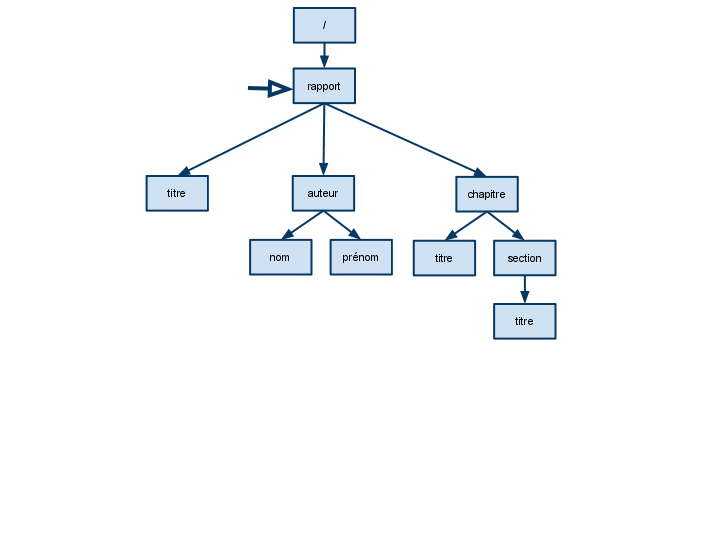
\includegraphics[width=0.7\textwidth]{img/XMLa.png}\\
	        
	        On recherche dans l'arbre XSLT l'élément "template" dont l'attribut "match" vaut "rapport"
	        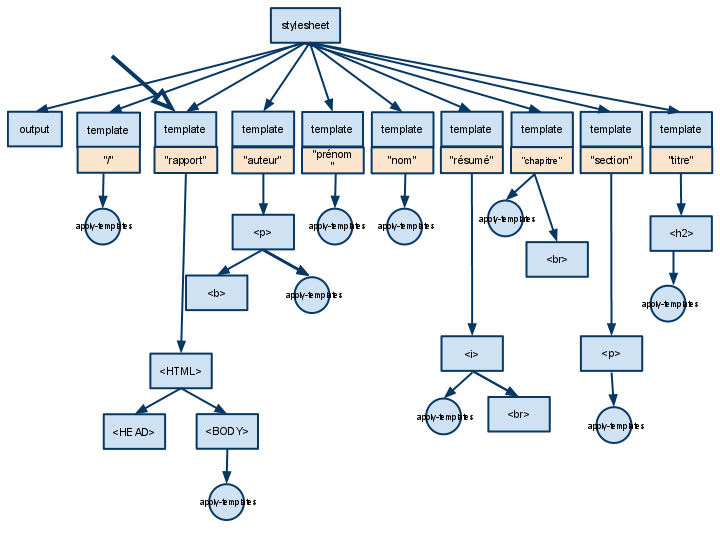
\includegraphics[width=0.7\textwidth]{img/XSLTa.png}\\
	        
	        On recopie les éléments fils de cette élément
	        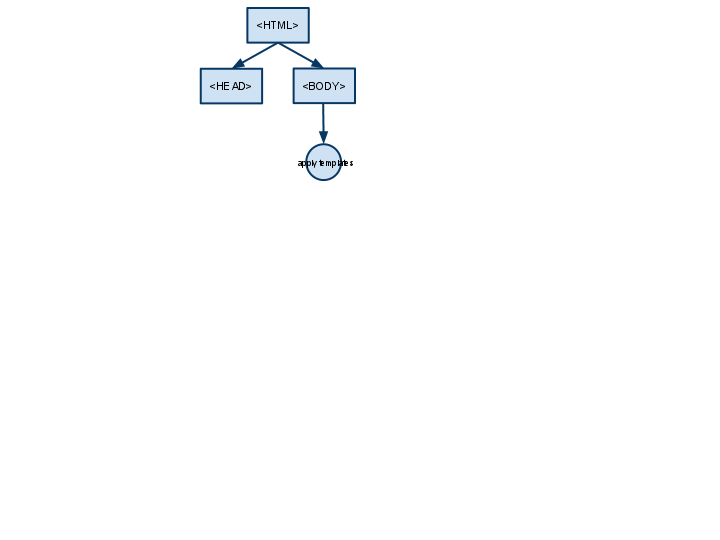
\includegraphics[width=0.7\textwidth]{img/HTMLa.png}\\
	        
	        On remarque que cette arbre à une feuille "apply-templates". On retourne donc sur l'arbre XML et on pointe sur le premier fils de "rapport" soit "titre"
	        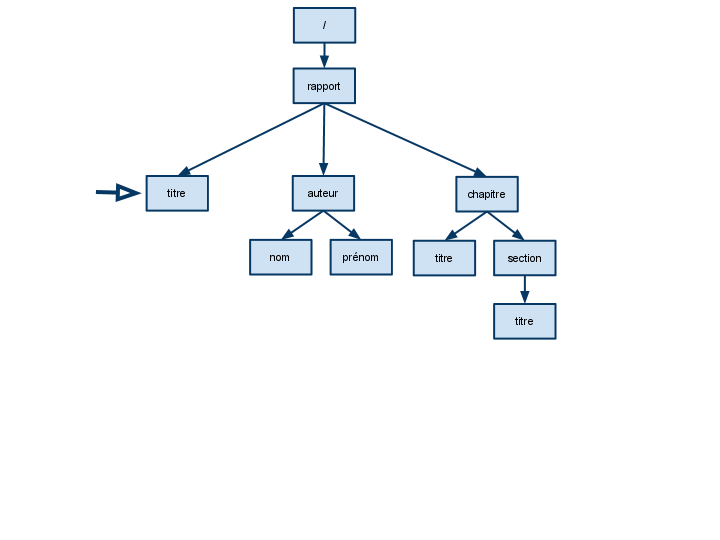
\includegraphics[width=0.7\textwidth]{img/XMLb.png}\\
	        
	        On recherche dans l'arbre XSLT l'élément "template" dont l'attribut "match" vaut "titre"
	        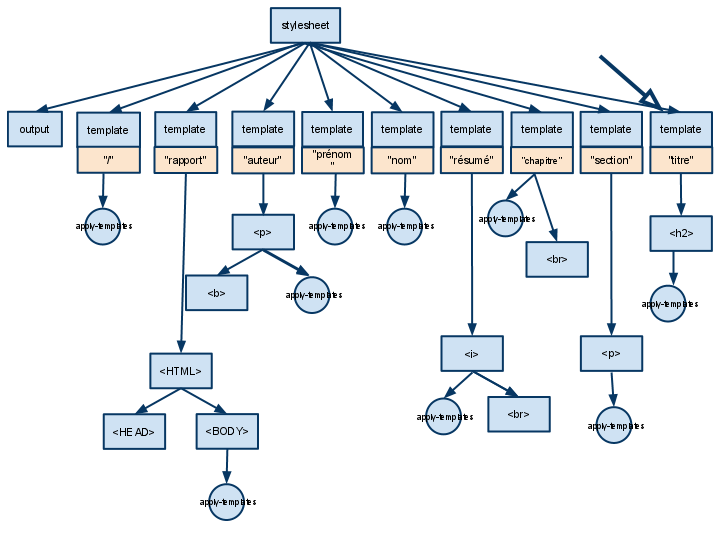
\includegraphics[width=0.7\textwidth]{img/XSLTb.png}\\
	        
	        On recopie les éléments fils de cette élément
	        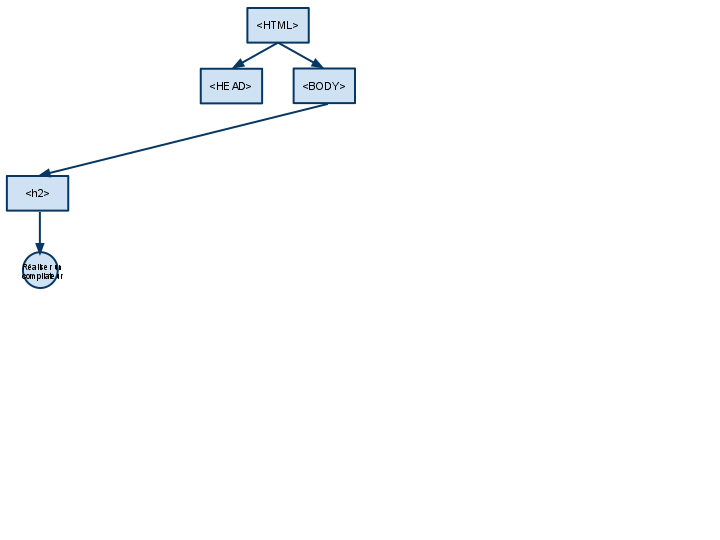
\includegraphics[width=0.7\textwidth]{img/HTMLb.png}\\
	        
	        Et ainsi de suite jusqu'à l'arbre suivant : 
	        On recherche dans l'arbre XSLT l'élément "template" dont l'attribut "match" vaut "rapport"
	        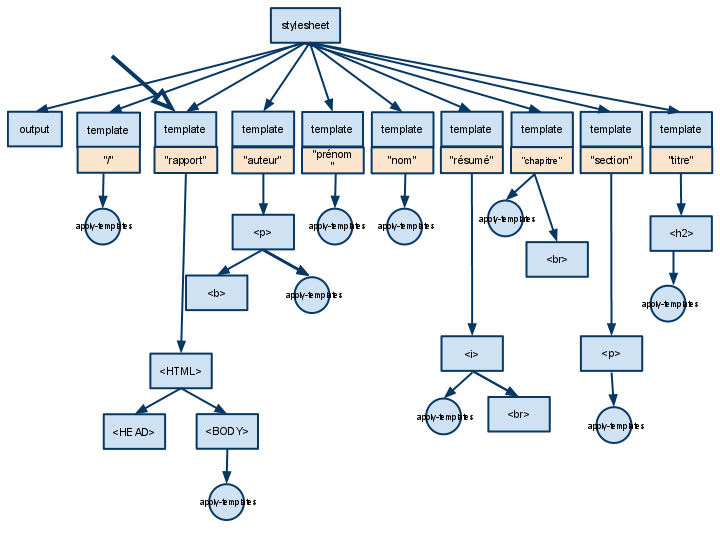
\includegraphics[width=0.7\textwidth]{img/XSLTa.png}\\
	        
	        On recopie les éléments fils de cette élément
	        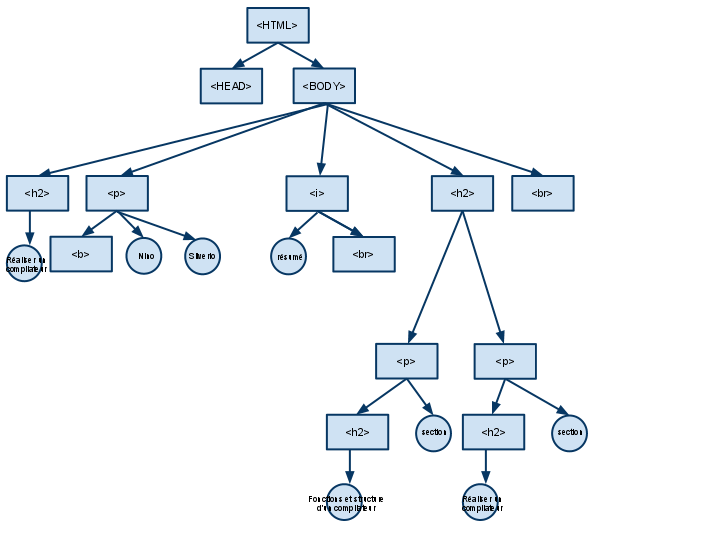
\includegraphics[width=0.7\textwidth]{img/ArbreHTML.png}
	    \end{center}
